% !TEX root = report.tex
\section{Introduction}


\subsection{Basic definition of database system}

In database systems, a \textbf{database} is a collection of tables, and each \textbf{table} stores one coherent dataset. Each row of a table represents a single data point and each column represents an attribute of the data. Theoretically speaking, a table is merely a mathematical \textbf{relation} over one or more sets of scalar values (numbers, strings, etc.) and each row of the table is a \textbf{tuple} (or an element) in such relation.

For the sake of keeping our explanation simple, the relationship of data across different tables can be expressed by declaring \textbf{keys} (usually referred as IDs) as explicit columns in the table. Each row of a table may have a \textbf{primary key} declared as an anchor point to which other tables can refer to with \textbf{foreign keys}. In practice, since integers can be used as keys, it is sufficient to portray keys no different than other scalar values. Therefore, we omit the keys from our discussion for the rest of this project.

\smallskip
\marginhead{First example of database}
For example, let us say that we would like to construct a database to store information of four students: Alice, Bob, Carol, and David. The database must contain their personal data (e.g. year of birth) as well as a network graph representing their friendship relation. One possibility is that we create two tables, described below.

\newrobustcmd\nameA{\field{Name\hrsp{}A}}
\newrobustcmd\nameB{\field{Name\hrsp{}B}}
\newrobustcmd\personaldata{\rel{PersonalData}(\field{Name},\field{BirthYear})}
\newrobustcmd\friendship{\rel{Friendship}(\nameA,\nameB)}

\begin{itemize}[topsep=0.5pc,itemsep=0.25pc]
    \item  $\personaldata$: a two-column table containing each student's name and year of birth;
    \item  $\friendship$: a (possibly non-symmetric) two-column table where each row contains names and only names of two students who are friends of each other.
\end{itemize}
An example of an instance of such database are shown in \autoref{tab:age} and \autoref{tab:friend}, and the visualization is shown in \autoref{fig:alicebob}.

\smallskip
\begin{table}[!h]
    \small\centering
    \begin{minipage}{0.45\linewidth}
        \centering
        \begin{tabular}{ll}
            \toprule
            \field{Name} & \field{BirthYear} \\
            \midrule
            \str{Alice} & \val{1994} \\
            \str{Bob} & \val{1995} \\
            \str{Carol} & \val{1994} \\
            \str{David} & \val{1993} \\
            \bottomrule
        \end{tabular}
        \caption{Table \rel{PersonalData} with four students: Alice, Bob, Carol, and David, and their corresponding year of birth.}
        \label{tab:age}
    \end{minipage}
    \begin{minipage}{0.45\linewidth}
        \centering
        \begin{tabular}{ll}
            \toprule
            \nameA & \nameB \\
            \midrule
            \str{Alice} & \str{Bob} \\
            \str{Bob} & \str{Carol} \\
            \str{Alice} & \str{Carol} \\
            \str{Carol} & \str{David} \\
            \bottomrule
        \end{tabular}
        \caption{Table \rel{Friendship} showing that Alice, Bob, and Carol know each other, but David knows only Carol.}
        \label{tab:friend}
    \end{minipage}
\end{table}
\begin{figure}[!h]
    \small\centering
    \begin{minipage}[b]{0.35\linewidth}
        \caption{The visualization of data in the table \rel{PersonalData} and \rel{Friendship}.}
        \label{fig:alicebob}
    \end{minipage}
    \begin{minipage}[b]{0.55\linewidth}
        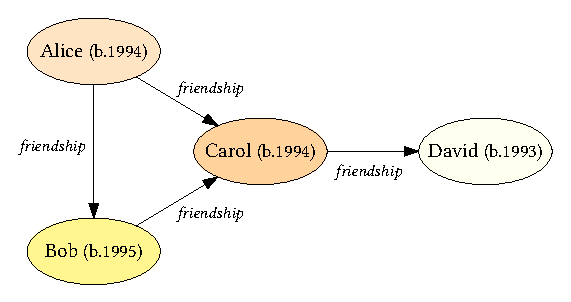
\includegraphics[width=0.8\linewidth]{figures/alicebob.eps}
    \end{minipage}
\end{figure}

\newpage
\subsection{Database query model}

One of the most basic database function is the \textbf{query} function, i.e., the process of fetching the stored data from the database. SQL model is an example of one of the most practical query model adopted in industry. Nonetheless, it is also useful to discuss theoretical query models (such as \textbf{relational calculus} and \textbf{relational algebra}) in order to gain a better understanding of database query models.

\marginhead{Definition of Domain Relational Calculus}In this report, we mainly discuss one particular variant of relational calculus query model, namely the \textbf{domain relational calculus} (\textsc{drc}). In this model,
\begin{itemize}[topsep=0.5pc,itemsep=0.25pc]
    \item  We use set comprehension notation (i.e., set defined by a predicate) to construct a query result. Such predicate must be in first-order logic.
    \item  Each identifier in the set comprehension must represent a scalar value in the database (as opposed to representing a tuple in tuple relational calculus).
\end{itemize}

\phantomsection
\label{psec:table-name-pred}
\marginhead{Table names as predicates}
As part of the predicate in set comprehension, the following notation regarding the existence of a tuple in a database table is allowed.

\begin{notation}
    Suppose that $R$ is a database table with $m$ columns. Let $\boldsymbol{x} = \langle x_1, x_2, \ldots, x_m \rangle$ be an $m$-tuple, where each $x_i$ represents a scalar value. Then $R(\boldsymbol{x})$ denotes a predicate whose value is true \emph{if and only if} the table $R$ contains the tuple $\boldsymbol{x}$. Sometimes we also write $R(x_1, x_2, \ldots, x_m)$ directly instead.
\end{notation}

For example, based on the data from \autoref{tab:age}, we could say that $\rel{PersonalData}(\str{Alice}, \val{1994})$ is true whereas $\rel{PersonalData}(\str{Bob}, \val{1993})$ is false.

\marginhead{Examples of \textnormal{\textsc{drc}} queries}
Here are some examples of \textsc{drc} queries.

\smallskip
\begin{example}
    Suppose that we want to obtain all students and their year of birth who were born \emph{strictly} before \val{1995} (using the database table $\personaldata$ as described in \autoref{tab:age}). We use the following \textsc{drc} query.
    \[
        Q_\text{\,before\,\val{1995}} = \{\var{name}, \var{year} \mid
            \rel{PersonalData}(\var{name}, \var{year}) \wedge (\var{year} < \val{1995})\}
    \]
    This query returns a set of three tuples: $\{(\str{Alice},\val{1994}),(\str{Carol},\val{1994}),(\str{David},\val{1993})\}$.
\end{example}

\begin{example}
    Suppose that we want to obtain all friends of Bob (based on the database table $\friendship$ from \autoref{tab:friend}). We use the following \textsc{drc} query.
    \[
        Q_\text{\,Bob's\,friend} = \{\var{name} \mid
            \rel{Friendship}(\var{name}, \str{Bob}) \vee
            \rel{Friendship}(\str{Bob}, \var{name})\}
    \]
    This query returns a set of two elements: $\{\str{Alice},\str{Carol}\}$. \emph{Note that we sometimes omit the tuple notation when it contains only a single column.}
\end{example}

\newpage
\begin{example}
    Suppose that we want to obtain all pairs of students who share a common friend using the same data as above. We use the following query.
    \begin{align*}
        Q_\text{\,friend\,of\,friend} = \{ x, y \mid (x < y) \wedge \exists z[
                &(\rel{Friendship}(x, z) \vee \rel{Friendship}(z, x)) \\
                &\quad\wedge (\rel{Friendship}(y, z) \vee \rel{Friendship}(z, y))
            ]\}
    \end{align*}
    This query would return $\{(\str{Alice},\str{Bob}),(\str{Alice},\str{Carol}),(\str{Bob},\str{Carol}),(\str{Alice},\str{David}),$ $(\str{Bob},\str{David})\}$. \emph{This query utilizes the existential quantification in first-order logic to represent a friend in common between two students. Also assume that $<$ does a lexicographical comparison of two strings.}
\end{example}

\medskip
\phantomsection
\label{psec:explicit-domain}
Notice how the domain for variables (such as \var{name} and \var{year}) are not explicit in the query. This is okay because predicates \rel{PersonalData} and \rel{Friendship} provides the \emph{finite bound} of what could be in the result of the query. We discuss this in more depth in the next subsection.


\subsection{Safety in \textsc{drc} queries}

\marginhead{Motivated example of unsafe queries}
\noindent
Let us consider the query $Q_\text{\,before\,\val{1995}}$ from above once again. You may have noticed that, at least in the paradigm of database systems, it would \emph{not} make practical sense to make such query but \emph{without} the predicate $\rel{PersonalData}(\var{name}, \var{year})$. If it was the case, then the result of the query would also have included tuples that are \emph{not} from the table \rel{PersonalData} in order to be consistent with the mathematical definition of set notation.

More concretely, the result of
\[
    Q^*_\text{\,before\,\val{1995}} = \{\var{name}, \var{year} \mid
        \var{year} < \val{1995}\}
\]
would change depending on what is defined as the scope or the domain of the scalar values. For example, if all nonempty strings are allowed for student names, and all integers are allowed for year of birth, then $(\str{Eve}, \val{-80})$ would be part of the query result. However, if the domain only allows positive integers for year of birth, then the same tuple would \emph{not} appear in the result.

\marginhead{Definition of safe vs. unsafe query}
We call queries like $Q^*_\text{\,before\,\val{1995}}$ \textbf{unsafe} as their result changes when the domain changes (i.e., results are \textbf{domain-dependent}). On the other hand, queries such as $Q_\text{\,before\,\val{1995}}$ and $Q_\text{\,Bob's\,friend}$ are examples of \textbf{safe} queries because the result of the query is always the same no matter what the scope of the domain is. In other words, their results rely only on data in the database. See Chapter 5 of \emph{Foundations of Databases} \cite[p.~75]{Abiteboul:1995:FDL:551350} for more information.

The concept of domain-dependency was summarized by Fagin in his paper \cite{Fagin:1982:HCD:322344.322347} and it was historically different from the \emph{original} meaning of safety of query formulae as introduced by Ullman \cite{Ullman:1983:PDS:538906}. For this project, we adopt a certain assumption \cite{Abiteboul:1988:inria-00075707} so we refer to a query as \textbf{safe} \emph{interchangeably} with the term \textbf{domain-independent}.

\newpage
\marginhead{More examples of unsafe queries}
Now let us consider a few more examples of unsafe queries. Assume that we have a database table $\rel{Follows}(\field{fan}, \field{idol})$ representing the fact that \field{fan} is following \field{idol} on a social network. Consider the following queries in \textsc{drc}.

\smallskip
\begin{example}
    \label{ex:not-follow}
    \[
        Q_\text{\,not\,following\,Alice} =
            \{ x \mid \neg\,\rel{Follows}(x, \str{Alice}) \}
    \]
    The first query, $Q_\text{\,not\,following\,Alice}$, returns a set of all people who did not follow Alice. It is unsafe because, for some database instance (such as when no one follows Alice), the result of the query will be every person within the domain. Hence, the result would be domain-dependent.
\end{example}

\begin{example}
    \[
        Q_\text{\,weird\,pairing} =
            \{ x, y \mid \rel{Follows}(x, \str{Alice}) \vee \rel{Follows}(y, \str{Bob}) \}
    \]
    The second query, $Q_\text{\,weird\,pairing}$, returns a set of pairs of people such that the first person follows Alice, or that the second person follows Bob. This query is also not safe. One counterexample is that no one follows Alice but Alice is the only person who follows Bob. Then $(x, \str{Alice})$ will appear in result for every $x$ in the domain of people, and thus is domain-dependent.
\end{example}

\begin{example}
    \label{ex:follow-all}
    \[
        Q_\text{\,follows\,all} =
            \{ x \mid \forall y[\rel{Follows}(x, y)] \}
    \]
    The third query $Q_\text{\,follows\,all}$ returns a set of people who follows everyone in the domain. Notice how the result for this query is guaranteed to be bounded even if the domain was infinite. However, suppose that Alice follows everyone in the domain $D_1$. If the domain $D_2$ is defined as $D_2 = D_1 \cup \{\str{Bob}\}$ where $\str{Bob} \not\in D_1$, then Alice would appear in the result when the domain $D_1$ is used, but would \emph{not} if $D_2$ is used. Therefore, query $Q_\text{\,follows\,all}$ is domain-dependent.
\end{example}


\subsection{Project goal and previous work}
\label{sub:goal}

The goal for this project is to study and analyze the safety of a query in \textsc{drc} model for a specified database schema using Alloy Analyzer (introduced in the next section). Specifically,

\begin{quote}
    \makebox[0pt][r]{``}Given a database schema $S$ and a query $Q$, does there exist a database instance under two \emph{distinct} domains $D_1$ and $D_2$ such that the respective results $R_1$ and $R_2$ differ. If so, then the query $Q$ is considered unsafe; otherwise it is safe.''
\end{quote}

The verification of data models using Alloy Analyzer has been investigated in prior work, including the data models whose specifications are in relational database schemata \cite{Cunha:2009:MAS:1685167.1685438} and other specification language such as \textsc{ora-ss} \cite{Wang:2006:VOD:1129030.1129454}.
The verification of data models in the context of web applications has also been studied \cite{Nijjar:2011:BVR:2001420.2001429,Nijjar:2015:DMP:2820114.2699691}. However, none of them involved the modeling of database relational queries.
Also note that we traditionally use Codd's Theorem \cite{codd1972relational} to verify whether a \textsc{drc} query is safe by providing an equivalent relational algebra query statement, which is outside the scope of this project.

Although relational calculus is not a practical way to make a query to the database, this project should provide an insight into the fundamental concepts of database theory as well as provide us a framework to help us on determining whether a \textsc{drc} query is safe, a task usually tediously done by humans due to its complexity.
